\documentclass[12pt]{article}

%%%%%%%%%%%%%%%%%%%%%%%%%%%%%%%%%%%%%%%%%%%%%
%%%%%%%%%%%%%%%% PACKAGES %%%%%%%%%%%%%%%%%%%
%%%%%%%%%%%%%%%%%%%%%%%%%%%%%%%%%%%%%%%%%%%%%

\usepackage[inner=2.1cm, bottom=1.5cm, top=1.5cm, outer=2.1cm,
  headheight=24pt, % as per the warning by fancyhdr
  includehead,includefoot,
  heightrounded]{geometry}
% Set the font
\usepackage{helvet}
\renewcommand{\familydefault}{\sfdefault}
% bitfield
\usepackage{bytefield}
% urls
\usepackage[hidelinks]{hyperref}
% disable indent
\usepackage[skip=1em, indent=0pt]{parskip}
% shifted environment
\newenvironment{content}%
  {\list{}{\leftmargin=1.5cm}\item[]}%
  {\endlist}
% cell color
\usepackage[table, dvipsnames]{xcolor}
% drawings
\usepackage{tikz}
\usepackage{pgfplots}
\pgfplotsset{compat=1.18}
\usetikzlibrary{shapes.geometric,angles,quotes}
\usetikzlibrary{arrows.meta}
\usetikzlibrary{positioning}
\usetikzlibrary{babel}
\usetikzlibrary{fit}
\usetikzlibrary{angles, quotes}
\tikzset{
% Define standard arrow tip
>={Latex[scale=1.25]}
}
\usepackage{tikz-layers}
\usepackage{tikz-timing}
\usetikztiminglibrary[rising arrows]{clockarrows}
\usetikztiminglibrary{either}
\usetikztiminglibrary{overlays}
% floating figures
\usepackage{float}
% do computations
\usepackage{calc}
% advanced tables
\usepackage{makecell}
\usepackage{tabularx}
\usepackage{xltabular}
\newcolumntype{Y}{>{\centering\arraybackslash}X}
\usepackage{multirow}
\usepackage{graphicx}
% no title at the end of pages
\usepackage[nobottomtitles]{titlesec}

%%%%%%%%%%%%%%%%%%%%%%%%%%%%%%%%%%%%%%%%%%%%%%
%%%%%%%%%%%%%%%% Variables %%%%%%%%%%%%%%%%%%%
%%%%%%%%%%%%%%%%%%%%%%%%%%%%%%%%%%%%%%%%%%%%%%

% VARIABLES
\def\version{1.0.0-draft1}
\def\parent{Educational Computer Architecture Platform 5}
\def\project{ECAP5-DPROC RISC-V processor}
\def\title{Architecture Document}


%%%%%%%%%%%%%%%%%%%%%%%%%%%%%%%%%%%%%%%%%%%%%%%%%%
%%%%%%%%%%%%%%%% Configuration %%%%%%%%%%%%%%%%%%%
%%%%%%%%%%%%%%%%%%%%%%%%%%%%%%%%%%%%%%%%%%%%%%%%%%

\setlength{\tabcolsep}{10pt}
\renewcommand{\arraystretch}{1.5}
% Functional requirement environment
\newlength{\reqtablelength}
\setlength{\reqtablelength}{0.9\textwidth}
\newcommand{\reqcolor}{blue!20!gray}
\newcommand{\req}[3]{
  \begin{center}
  {
    \footnotesize
    \begin{tabularx}{\reqtablelength}{|l|X|}
      \hline
      \cellcolor{\reqcolor!30}\textbf{ID} & #1\\
      \hline
      \cellcolor{\reqcolor!15}\textbf{Description} & \cellcolor{\reqcolor!5}{#2} \\
      \hline
      \cellcolor{\reqcolor!15}\textbf{Refers to} & \cellcolor{\reqcolor!5}\makecell[l]{#3} \\
      \hline
    \end{tabularx}
  }
  \end{center}
}
\newcommand{\reqwithratio}[4]{
  \begin{center}
  {
    \footnotesize
    \begin{tabularx}{\reqtablelength}{|l|X|}
      \hline
      \cellcolor{\reqcolor!30}\textbf{ID} & #1\\
      \hline
      \cellcolor{\reqcolor!15}\textbf{Description} & \cellcolor{\reqcolor!5}{#2} \\
      \hline
      \cellcolor{\reqcolor!15}\textbf{Rationale} & \cellcolor{\reqcolor!5}#3 \\
      \hline
      \cellcolor{\reqcolor!15}\textbf{Refers to} & \cellcolor{\reqcolor!5}#4 \\
      \hline
    \end{tabularx}
  }
  \end{center}
}
% User requirement 
\newlength{\ureqtablelength}
\setlength{\ureqtablelength}{0.9\textwidth}
\newcommand{\ureqcolor}{blue!20!gray}
\newcommand{\ureq}[2]{
  \begin{center}
  {
    \footnotesize
    \begin{tabularx}{\ureqtablelength}{|l|X|}
      \hline
      \cellcolor{\ureqcolor!30}\textbf{ID} & #1\\
      \hline
      \cellcolor{\ureqcolor!15}\textbf{Description} & \cellcolor{\ureqcolor!5}#2 \\
      \hline
    \end{tabularx}
  }
  \end{center}
}
% External interface requirement
\newlength{\ireqtablelength}
\setlength{\ireqtablelength}{0.9\textwidth}
\newcommand{\ireqcolor}{blue!20!gray}
\newcommand{\ireq}[3]{
  \begin{center}
  {
    \footnotesize
    \begin{tabularx}{\ireqtablelength}{|l|X|}
      \hline
      \cellcolor{\ireqcolor!30}\textbf{ID} & #1\\
      \hline
      \cellcolor{\ireqcolor!15}\textbf{Description} & \cellcolor{\ireqcolor!5}#2 \\
      \hline
      \cellcolor{\ireqcolor!15}\textbf{Refers to} & \cellcolor{\ireqcolor!5}\makecell[l]{#3} \\
      \hline
    \end{tabularx}
  }
  \end{center}
}
\newcommand{\ireqwithratio}[4]{
  \begin{center}
  {
    \footnotesize
    \begin{tabularx}{\ireqtablelength}{|l|X|}
      \hline
      \cellcolor{\ireqcolor!30}\textbf{ID} & #1\\
      \hline
      \cellcolor{\ireqcolor!15}\textbf{Description} & \cellcolor{\ireqcolor!5}#2 \\
      \hline
      \cellcolor{\ireqcolor!15}\textbf{Rationale} & \cellcolor{\ireqcolor!5}\makecell[l]{#3} \\
      \hline
      \cellcolor{\ireqcolor!15}\textbf{Refers to} & \cellcolor{\ireqcolor!5}\makecell[l]{#4} \\
      \hline
    \end{tabularx}
  }
  \end{center}
}

% Configure headers and footers
\usepackage{fancyhdr}
\renewcommand{\headrulewidth}{1pt}
\renewcommand{\footrulewidth}{1pt}
\renewcommand{\headruleskip}{4pt}
\renewcommand{\footruleskip}{4pt}
\fancyhead{}\fancyfoot{}
\fancyhead[HL]{\scriptsize{\textbf{\parent} \\
\project}}
\fancyhead[HR]{\scriptsize{Page \thepage \\
}}
\fancyfoot[FL]{\scriptsize{\title}}
\fancyfoot[FR]{\scriptsize{Issue Date: \today}}
\fancyfoot[FC]{\scriptsize{\vspace{1em}\textit{Revision \version}}}

%%%%%%%%%%%%%%%%%%%%%%%%%%%%%%%%%%%%%%%%%%%%
%%%%%%%%%%%%%%%% Content %%%%%%%%%%%%%%%%%%%
%%%%%%%%%%%%%%%%%%%%%%%%%%%%%%%%%%%%%%%%%%%%

\begin{document}
\input{docs/arch/content/0_titlepage}
\pagestyle{fancy}
\normalsize
\tableofcontents
\newpage
\section{Introduction}
  \subsection{Purpose}

    \begin{content}
        This documents aims at defining the requirements for ECAP5-DPROC as well as describing its architecture. Both user and product requirements will be covered.
      \end{content}

  \subsection{Intended Audience and Use}

    \begin{content}
        This document targets hardware engineers who shall implement ECAP5-DPROC by refering to the described architecture. It is also intended for system engineers working on the integration of ECAP5-DPROC in ECAP5. Finally, this document shall be used as a technical reference by software engineers configuring ECAP5-DPROC through hardware-software interfaces.
      \end{content}

  \subsection{Product Scope}

    \begin{content}
        ECAP5-DPROC is an implementation of the RISC-V instruction set architecture targetting \textit{Educational Computer Architecture Platform 5} (ECAP5). It will provide the main means of software execution in ECAP5.
      \end{content}

  \subsection{Conventions}

    Requirements shall be described here.

    Requirement relationships :
    \begin{itemize}
        \item Composition
        \item Derivation
        \item Refinement
        \item Satisfy
        \item Verify
        \item Copy
      \end{itemize}

    The bit indexing shall be described somewhere.

    Byte size as well.

    Inputs missing from timing diagrams are considered low or undefined.

    Italic names are timing diagram parameters.

  \subsection{Definitions and Abbreviations}

    hardware-configurable

    software-configurable

  \subsection{References}

    \begin{center}
        \vspace{0.5em}
        \small
        \begin{tabularx}{0.9\textwidth}{|c|c|X|}
            \hline
            \cellcolor{gray!20}\textbf{Date} & \cellcolor{gray!20}\textbf{Version} & \cellcolor{gray!20}\textbf{Title} \\
            \hline
            December 13, 2019 & 20191213 & The RISC-V Instruction Set Manual Volume I: User-Level ISA \\
            \hline
            March 22, 2019 & 0.13.2 & RISC-V External Debug Support \\
            \hline
            June 22, 2010 & B.4 & WISHBONE System-on-Chip (SoC) Interconnection Architecture for Portable IP Cores \\
            \hline
          \end{tabularx}
        \vspace{0.5em}
      \end{center}

\newpage

\section{Overall Description}

\subsection{User needs}

\begin{content}
ECAP5 is the primary user for ECAP5-DPROC. ECAP5-DPROC could however be used as a standalone RISC-V processor. The following requirements define the user needs. 
\end{content}

\ureq{U\_INSTRUCTION\_SET\_01}{
  ECAP5-DPROC shall implement the RV32I instruction set.
}

\begin{content}
  In order to improve the usability of ECAP5-DPROC, it shall have a \textit{von Neumann} architecture as it only requires one memory interface.
\end{content}

\ureq{U\_MEMORY\_INTERFACE\_01}{
  ECAP5-DPROC shall access both instructions and data through a unique memory interface.
}

\ureq{U\_MEMORY\_INTERFACE\_02}{
  ECAP5-DPROC's unique memory interface shall be compliant with the AXI-Lite specification.
}

\ureq{U\_RESET\_01}{
  ECAP5-DPROC shall provide a signal which shall hold ECAP5-DPROC in a reset state while asserted.
}

\begin{content}
The polarity of the reset signal mentionned in \texttt{U\_RESET\_01} is not specified by the user.
\end{content}

\ureq{U\_BOOT\_ADDRESS\_01}{
  The address at which ECAP5-DPROC jumps after the reset signal is deasserted shall be hardware-configurable.
}

\begin{content}
The address mentionned in \texttt{U\_BOOT\_ADDRESS\_01} can be either configured through hardware signals or can be selected at compile-time.
\end{content}

\ureq{U\_HARDWARE\_INTERRUPT\_01}{
  ECAP5-DPROC shall provide an signal which shall interrupt ECAP5-DPROC's execution flow while asserted.
}

\ureq{U\_HARDWARE\_INTERRUPT\_02}{
  ECAP5-DPROC shall jump to a software-configurable address when it is interrupted.
}

\begin{content}
The memory address at which ECAP5-DPROC shall jump to when interrupted is not specified by the user.
\end{content}

\ureq{U\_DEBUG\_01}{
  ECAP5-DPROC shall be compliant with the RISC-V External Debug Support specification.
}

\begin{content}
There is no performance goal required by ECAP5 for ECAP5-DPROC as ECAP5 is an educational platform.
\end{content}

\subsection{Assumptions and Dependencies}

\begin{content}
Describe what the assumptions for the product are : Targeting the ecp5 family, based around opensource toolchains.
\end{content}

\section{Requirements}

\subsection{External Interface Requirements}

\begin{figure}[h!]
    \centering
    \scalebox{0.85}{
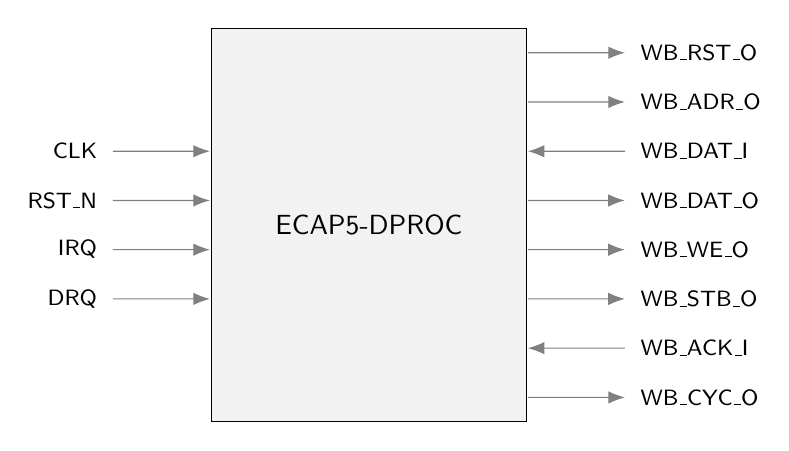
\begin{tikzpicture}[scale=1.25, draw=gray, inner sep=0, outer sep=0]
  \node[rectangle, draw=black,
    minimum height = 5cm,
    minimum width = 4cm,
    fill = gray!10] (box) at (0, 0) {ECAP5-DPROC};

  % left
  \node (lport1) at ([yshift=0.75cm]box.west) {};
  \node (lport2) at ([yshift=0.25cm]box.west) {};
  \node (lport3) at ([yshift=-0.25cm]box.west) {};
  \node (lport4) at ([yshift=-0.75cm]box.west) {};

  \draw[->] ([xshift=-1cm]lport1.center) node[left=0.2cm, anchor=east]{\footnotesize CLK} -- (lport1);
  \draw[->] ([xshift=-1cm]lport2.center) node[left=0.2cm, anchor=east]{\footnotesize RST\_N} -- (lport2);
  \draw[->] ([xshift=-1cm]lport3.center) node[left=0.2cm, anchor=east]{\footnotesize IRQ} -- (lport3);
  \draw[->] ([xshift=-1cm]lport4.center) node[left=0.2cm, anchor=east]{\footnotesize DRQ} -- (lport4);

  % right
  \node (rport4) at ([yshift=0.25cm]box.east) {};
  \node (rport3) at ([yshift=0.5cm]rport4.center) {};
  \node (rport2) at ([yshift=0.5cm]rport3.center) {};
  \node (rport1) at ([yshift=0.5cm]rport2.center) {};

  \node (rport5) at ([yshift=-0.25cm]box.east) {};
  \node (rport6) at ([yshift=-0.5cm]rport5.center) {};
  \node (rport7) at ([yshift=-0.5cm]rport6.center) {};
  \node (rport8) at ([yshift=-0.5cm]rport7.center) {};

  \draw[<-] ([xshift=1cm]rport1.center) node[right=0.2cm, anchor=west]{\footnotesize WB\_RST\_O} -- (rport1);
  \draw[<-] ([xshift=1cm]rport2.center) node[right=0.2cm, anchor=west]{\footnotesize WB\_ADR\_O} -- (rport2);
  \draw[->] ([xshift=1cm]rport3.center) node[right=0.2cm, anchor=west]{\footnotesize WB\_DAT\_I} -- (rport3);
  \draw[<-] ([xshift=1cm]rport4.center) node[right=0.2cm, anchor=west]{\footnotesize WB\_DAT\_O} -- (rport4);
  \draw[<-] ([xshift=1cm]rport5.center) node[right=0.2cm, anchor=west]{\footnotesize WB\_WE\_O} -- (rport5);
  \draw[<-] ([xshift=1cm]rport6.center) node[right=0.2cm, anchor=west]{\footnotesize WB\_STB\_O} -- (rport6);
  \draw[->] ([xshift=1cm]rport7.center) node[right=0.2cm, anchor=west]{\footnotesize WB\_ACK\_I} -- (rport7);
  \draw[<-] ([xshift=1cm]rport8.center) node[right=0.2cm, anchor=west]{\footnotesize WB\_CYC\_O} -- (rport8);
\end{tikzpicture}
}

    \caption{Schematic view of the external interface of ECAP5-DPROC}
    \label{fig:externalinterface}
\end{figure}

\begin{table}[H]
  \centering
  {
\footnotesize
\begin{tabularx}{0.9\textwidth}{|l|c|c|X|}
  \hline
  \cellcolor{gray!20}\textbf{NAME} & \cellcolor{gray!20}\textbf{TYPE} & \cellcolor{gray!20}\textbf{WIDTH} & \cellcolor{gray!20}\textbf{DESCRIPTION} \\
  \hline
  CLK & I & 1 & Clock input. \\
  \hline
  RST\_N & I & 1 & Hardware reset. Active low. \\
  \hline
  IRQ & I & 1 & External interrupt request. \\
  \hline
  DRQ & I & 1 & Debug request. \\
  \hline
\end{tabularx}
}

  \caption{ECAP5-DPROC control signals}
  \label{tab:control-interface}
\end{table}

\begin{table}[H]
  \centering
  {
\footnotesize
\begin{tabularx}{\reqtablelength}{|l|c|c|X|}
  \hline
  \cellcolor{gray!20}\textbf{NAME} & \cellcolor{gray!20}\textbf{TYPE} & \cellcolor{gray!20}\textbf{WIDTH} & \cellcolor{gray!20}\textbf{DESCRIPTION} \\
  \hline
  \multicolumn{4}{|l|}{\textbf{READ ADDRESS BUS}} \\
  \hline
  ARADDR & O & 32 & Read address. \\
  \hline
  ARVALID & O & 1 & Read address valid. \\
  \hline
  ARREADY & I & 1 & Read address ready. \\ 
  \hline
  \multicolumn{4}{|l|}{\textbf{READ DATA BUS}} \\
  \hline
  RDATA & I & 32 & Read data. \\
  \hline
  RRESP & I & 2 & Read response. \\
  \hline
  RVALID & I & 1 & Read valid. \\
  \hline
  RREADY & O & 1 & Read ready. \\ 
  \hline
  \multicolumn{4}{|l|}{\textbf{WRITE ADDRESS BUS}} \\
  \hline
  AWADDR & O & 32 & Write address. \\
  \hline
  AWVALID & O & 1 & Write address valid. \\
  \hline
  AWREADY & I & 1 & Write address ready \\
  \hline
  \multicolumn{4}{|l|}{\textbf{WRITE DATA BUS}} \\
  \hline
  WDATA & O & 32 & Write data. \\
  \hline
  WSTRB & O & 4 & Write strobes. \\
  \hline
  \multicolumn{4}{|l|}{\textbf{WRITE RESPONSE BUS}} \\
  \hline
  BRESP & I & 2 & Write response. \\
  \hline
  BVALID & I & 1 & Write response valid. \\
  \hline
  BREADY & O & 1 & Response ready. \\
  \hline
\end{tabularx}
}

  \caption{ECAP5-DPROC memory interface signals}
  \label{tab:memory-interface}
\end{table}

\ireq{I\_CLK\_01}{
  All inputs and outputs of ECAP5-DPROC shall belong to CLK's clock domain.
}{}

\ireq{I\_RESET\_01}{
  The RST\_N signal shall hold ECAP5-DPROC in a reset state while asserted.
}{
  U\_RESET\_01
}

\ireq{I\_RESET\_02}{
  RST\_N polarity shall be active low.
}{}

\ireq{I\_IRQ\_01}{
  ECAP5-DPROC shall jump to a software-configurable address when input IRQ is asserted.
}{
  U\_HARDWARE\_INTERRUPT\_01, U\_HARDWARE\_INTERRUPT\_02
}

\ireq{I\_DIRQ\_01}{
  TBD
}{}

\ireq{I\_MEMORY\_INTERFACE\_01}{
  Signals from table \ref{tab:memory-interface} shall be compliant with the AXI-Lite specification.
}{
  U\_MEMORY\_INTERFACE\_02
}

\begin{content}
  Behavioral specification for symbols in table \ref{tab:memory-interface} is outlined in the functional requirements section, subsection \ref{spec-memory-interface}.
\end{content}

\subsection{Functional Requirements}

\subsubsection{Register file}

\req{F\_REGISTERS\_01}{
  ECAP5-DPROC shall implement 31 user-accessible general purpose registers ranging from \texttt{x0} to \texttt{x31}.
}{U\_INSTRUCTION\_SET\_01}

\req{F\_REGISTERS\_02}{
  Register \texttt{x0} shall be hardwired to the constant zero.
}{U\_INSTRUCTION\_SET\_01}

\req{F\_REGISTERS\_03}{
  ECAP5-DPROC shall implement a \texttt{pc} user-accessible register storing the address of the current instruction.
}{U\_INSTRUCTION\_SET\_01}

\subsubsection{Instruction decoding}

\begin{content}
  Figure \ref{fig:instructionencoding} outlines the different instruction encodings for the RV32I instruction set. The \texttt{opcode} parameter is a unique identifier for each instruction. The instruction encoding is infered from the opcode as there can only be one encoding per opcode.
\end{content}

\begin{figure}[h!]
    \centering
    \vspace{0.5em}

\hspace{2em}
\scalebox{0.9}{
\begin{bytefield}[
    bitwidth=1.1em, 
    endianness=big, 
    bitformatting={\scriptsize}, 
    boxformatting={\centering\footnotesize},
    rightcurly=., rightcurlyspace=5pt
]{32}
  \bitheader{0,6,7,8,11,12,14,15,19,20,24,25,31} \\
  \begin{rightwordgroup}{\footnotesize R-type}
    \bitbox{7}{funct7}
    \bitbox{5}{rs2}
    \bitbox{5}{rs1}
    \bitbox{3}{func3}
    \bitbox{5}{rd}
    \bitbox{7}{opcode}
  \end{rightwordgroup}
  \\[2ex]
  \begin{rightwordgroup}{\footnotesize I-type}
    \bitbox{12}{imm[11:0]}
    \bitbox{5}{rs1}
    \bitbox{3}{func3}
    \bitbox{5}{rd}
    \bitbox{7}{opcode}
  \end{rightwordgroup}
  \\[2ex]
  \begin{rightwordgroup}{\footnotesize S-type}
    \bitbox{7}{imm[11:5]}
    \bitbox{5}{rs2}
    \bitbox{5}{rs1}
    \bitbox{3}{func3}
    \bitbox{5}{imm[4:0]}
    \bitbox{7}{opcode}
  \end{rightwordgroup}
  \\[2ex]
  \begin{rightwordgroup}{\footnotesize B-type}
    \bitbox{1}{a}
    \bitbox{6}{imm[10:5]}
    \bitbox{5}{rs2}
    \bitbox{5}{rs1}
    \bitbox{3}{func3}
    \bitbox{4}{imm[4:1]}
    \bitbox{1}{b}
    \bitbox{7}{opcode}
  \end{rightwordgroup}
  \\[2ex]
  \begin{rightwordgroup}{\footnotesize U-type}
    \bitbox{20}{imm[31:12]}
    \bitbox{5}{rd}
    \bitbox{7}{opcode}
  \end{rightwordgroup}
  \\[2ex]
  \begin{rightwordgroup}{\footnotesize J-type}
    \bitbox{1}{c}
    \bitbox{10}{imm[10:1]}
    \bitbox{1}{b}
    \bitbox{8}{imm[31:12]}
    \bitbox{5}{rd}
    \bitbox{7}{opcode}
  \end{rightwordgroup}
\end{bytefield}
}

\vspace{0.25em}
\scalebox{0.7}{
\begin{tabularx}{0.8\textwidth}{Y Y Y}
a: imm[12] & b: imm[11] & c: imm[20]
\end{tabularx}
}

    \caption{Instruction encodings of the RV32I instruction set}
    \label{fig:instructionencoding}
\end{figure}

\paragraph{Immediate encoding}

\begin{content}
  Only one immediate value can be encoded in one instruction. The value can be reconstructed from fragments of the following format : imm[x] representing the x\textsuperscript{th} bit or imm[x:y] representing bits from the x\textsuperscript{th} to the y\textsuperscript{th} both included.
\end{content}

\req{F\_INSTR\_IMMEDIATE\_01}{
  Immediate values shall be sign-extended.
}{U\_INSTRUCTION\_SET\_01}

\begin{content}
  RV32I is called a Load/Store ISA, meaning that instructions inputs and outputs are passed through registers or through an instruction immediate. There are specific instructions for loading and storing data into memory.
\end{content}

\paragraph{Instruction inputs}

\req{F\_INSTR\_FIRST\_INPUT\_01}{
  Instructions encoded using the R-type, I-type, S-type and B-type shall take as their first input the value stored in the register designated by the \texttt{rs1} parameter.
}{U\_INSTRUCTION\_SET\_01}

\req{F\_INSTR\_FIRST\_INPUT\_02}{
  Instructions encoded using the U-type and J-type shall take as their first input the immediate value encoded in the instruction.
}{U\_INSTRUCTION\_SET\_01}

\req{F\_INSTR\_SECOND\_INPUT\_01}{
  Instructions encoded using the R-type, S-type and B-type shall take as their second input the value stored in the register designated by the \texttt{rs2} parameter.
}{U\_INSTRUCTION\_SET\_01}

\req{F\_INSTR\_SECOND\_INPUT\_02}{
  Instructions encoded using the I-type shall take as its second input the immediate value encoded in the instruction.
}{U\_INSTRUCTION\_SET\_01}

\req{F\_INSTR\_THIRD\_INPUT\_01}{
  Instructions encoded using the S-type and B-type shall take as their third input the immediate value encoded in the instruction.
}{U\_INSTRUCTION\_SET\_01}

\paragraph{Instruction outputs}

\req{F\_INSTR\_OUTPUT\_01}{
  Instructions encoded using the R-type, I-type, U-type and J-type shall store their result in the register designated by the \texttt{rd} parameter.
}{U\_INSTRUCTION\_SET\_01}

\req{F\_INSTR\_OUTPUT\_02}{
  Instructions encoded using the S-type and B-type do not produce any result.
}{U\_INSTRUCTION\_SET\_01}

\paragraph{Instruction variants}

\req{F\_INSTR\_VARIANT\_01}{
  Instructions encoded using the R-type, I-type, S-type and B-type shall use the \texttt{func3} parameter as a behavior variant selector.
}{U\_INSTRUCTION\_SET\_01}

\req{F\_INSTR\_VARIANT\_02}{
  Instructions encoded using the R-type shall use the \texttt{func7} parameter as a secondary behavior variant selector.
}{U\_INSTRUCTION\_SET\_01}

\paragraph{Opcodes}

\vspace{1em}
\begin{content}
  Table \ref{tab:opcodemap} outlines the different opcodes values of the RV32I instruction set. Cells marked as \textit{noimp} are for opcodes that are not implemented in ECAP5-DPROC.
\end{content}

\begin{table}[H]
  \centering
  \scalebox{0.8}{
\footnotesize
\begin{tabular}{|r|c|c|c|c|c|c|c|c|}
  \hline
  opcode[1:0] & \multicolumn{8}{|c|}{11} \\
  \hline
  opcode[4:2] & \multirow{2}{*}{000} & \multirow{2}{*}{001} & \multirow{2}{*}{010} & \multirow{2}{*}{011} & \multirow{2}{*}{100} & \multirow{2}{*}{101} & \multirow{2}{*}{110} & \multirow{2}{*}{111} \\
  \cline{1-1}
  opcode[6:5] & & & & & & & & \\
  \hline
  00 & LOAD & \cellcolor{gray!20}\textit{noimp} & \cellcolor{gray!20}\textit{noimp} & MISC-MEM & OP-IMM & AUIPC & \cellcolor{gray!20}\textit{noimp} & \cellcolor{gray!20}\textit{noimp} \\
  \hline
  01 & STORE & \cellcolor{gray!20}\textit{noimp} & \cellcolor{gray!20}\textit{noimp} & \cellcolor{gray!20}\textit{noimp} & OP & LUI & \cellcolor{gray!20}\textit{noimp} & \cellcolor{gray!20}\textit{noimp} \\
  \hline
  10 & \cellcolor{gray!20}\textit{noimp} & \cellcolor{gray!20}\textit{noimp} & \cellcolor{gray!20}\textit{noimp} & \cellcolor{gray!20}\textit{noimp} & \cellcolor{gray!20}\textit{noimp} & \cellcolor{gray!20}\textit{noimp} & \cellcolor{gray!20}\textit{noimp} & \cellcolor{gray!20}\textit{noimp} \\
  \hline
  11 & BRANCH & JALR & \cellcolor{gray!20}\textit{noimp} & JAL & SYSTEM & \cellcolor{gray!20}\textit{noimp} & \cellcolor{gray!20}\textit{noimp} & \cellcolor{gray!20}\textit{noimp} \\
  \hline
\end{tabular}
}

  \caption{Opcode values for the RV32I instruction set.}
  \label{tab:opcodemap}
\end{table}

\req{F\_OPCODE\_ENCODING\_01}{
  Instructions which use the LUI opcode shall be decoded as an U-type instruction.
}{U\_INSTRUCTION\_SET\_01}

\req{F\_OPCODE\_ENCODING\_02}{
  Instructions which use the AUIPC opcode shall be decoded as an U-type instruction.
}{U\_INSTRUCTION\_SET\_01}

\req{F\_OPCODE\_ENCODING\_03}{
  Instructions which use the JAL opcode shall be decoded as a J-type instruction.
}{U\_INSTRUCTION\_SET\_01}

\req{F\_OPCODE\_ENCODING\_04}{
  Instructions which use the JALR opcode shall be decoded as an I-type instruction.
}{U\_INSTRUCTION\_SET\_01}

\req{F\_OPCODE\_ENCODING\_05}{
  Instructions which use the BRANCH opcode shall be decoded as a B-type instruction.
}{U\_INSTRUCTION\_SET\_01}

\req{F\_OPCODE\_ENCODING\_06}{
  Instructions which use the LOAD opcode shall be decoded as an I-type instruction.
}{U\_INSTRUCTION\_SET\_01}

\req{F\_OPCODE\_ENCODING\_07}{
  Instructions which use the STORE opcode shall be decoded as a S-type instruction.
}{U\_INSTRUCTION\_SET\_01}

\req{F\_OPCODE\_ENCODING\_08}{
  Instructions which use the OP-IMM opcode shall be decoded as an I-type instruction.
}{U\_INSTRUCTION\_SET\_01}

\req{F\_OPCODE\_ENCODING\_09}{
  Instructions which use the OP opcode shall be decoded as a R-type instruction.
}{U\_INSTRUCTION\_SET\_01}

\req{F\_OPCODE\_ENCODING\_10}{
  Instructions which use the MISC-MEM opcode shall be decoded as an I-type instruction.
}{U\_INSTRUCTION\_SET\_01}

\req{F\_OPCODE\_ENCODING\_11}{
  Instructions which use the SYSTEM opcode shall be decoded as an I-type instruction.
}{U\_INSTRUCTION\_SET\_01}

\subsubsection{Instructions behaviors}

\paragraph{LUI}

\paragraph{AUIPC}

\paragraph{JAL}

\paragraph{JALR}

\paragraph{BEQ}

\paragraph{BNE}

\paragraph{BLT}

\paragraph{BGE}

\paragraph{BLTU}

\paragraph{BGEU}

\paragraph{LB}

\paragraph{LH}

\paragraph{LW}

\paragraph{LBU}

\paragraph{LHU}

\paragraph{SB}

\paragraph{SH}

\paragraph{SW}

\paragraph{ADDI}

\req{F\_ADDI\_01}{
  The ADDI behavior shall be applied the opcode is OP-IMM and when func3 is 0x0.
}{U\_INSTRUCTION\_SET\_01}

\req{F\_ADDI\_02}{
  The output of ADDI shall be the signed integer sum of its two inputs.
}{U\_INSTRUCTION\_SET\_01}

\req{F\_ADDI\_03}{
  The output of ADDI shall be truncated to 32-bits.
}{U\_INSTRUCTION\_SET\_01}

\paragraph{SLTI}

\req{F\_SLTI\_01}{
  The SLTI behavior shall be applied the opcode is OP-IMM and when func3 is 0x2.
}{U\_INSTRUCTION\_SET\_01}

\req{F\_SLTI\_02}{
  The output of SLTI shall be 1 when the signed value of its first input is lower that the signed value of its second input.
}{U\_INSTRUCTION\_SET\_01}

\paragraph{SLTIU}

\req{F\_SLTIU\_01}{
  The SLTIU behavior shall be applied the opcode is OP-IMM and when func3 is 0x3.
}{U\_INSTRUCTION\_SET\_01}

\req{F\_SLTIU\_02}{
  The output of SLTI shall be 1 when the unsigned value of its first input is lower that the unsigned value of its second input. It shall be 0 otherwise.
}{U\_INSTRUCTION\_SET\_01}

\paragraph{XORI}

\paragraph{ORI}

\paragraph{ANDI}

\paragraph{SLLI}

\paragraph{SRLI}

\paragraph{SRAI}

\paragraph{ADD}

\paragraph{SUB}

\paragraph{SLL}

\paragraph{SLT}

\paragraph{SLTU}

\paragraph{XOR}

\paragraph{SRL}

\paragraph{SRA}

\paragraph{OR}

\paragraph{AND}

\paragraph{FENCE}

\paragraph{ECALL}

\paragraph{EBREAK}

\subsubsection{Exceptions}

\req{F\_INSTR\_ADDR\_MISALIGNED\_01}{
  An Instruction Address Misaligned exception shall be raised when the target address of a taken branch or an unconditional jump if not four-byte aligned.
}{U\_INSTRUCTION\_SET\_01}


\subsubsection{Memory interface}
\label{spec-memory-interface}

\begin{content}
  Outline requirements to be compliant with the AXI-Lite specification.
\end{content}

\subsection{Nonfunctional Requirements}

\begin{content}
These can be : performance, safety, security, usability, scalability.
\end{content}

\newpage

\section{Functional Partitioning}

\begin{content}
  ECAP5-DPROC is built around a pipelined architecture with the following stages :
  \begin{itemize}
    \vspace{-0.5em}
    \item The instruction fetch stage loads the next instruction from memory.
    \vspace{-0.5em}
    \item The decode stage handles the instruction decoding to provide the next stage with the different instruction input values including reading from internal registers.
    \vspace{-0.5em}
    \item The execute stage implements instruction behaviors. This includes performing integer operations as well as accessing memory.
    \vspace{-0.5em}
    \item The write-back stage which handles storing instructions outputs to internal registers.
  \end{itemize}

\begin{figure}[h!]
    \centering
    \vspace{1em}
\scalebox{0.75}{
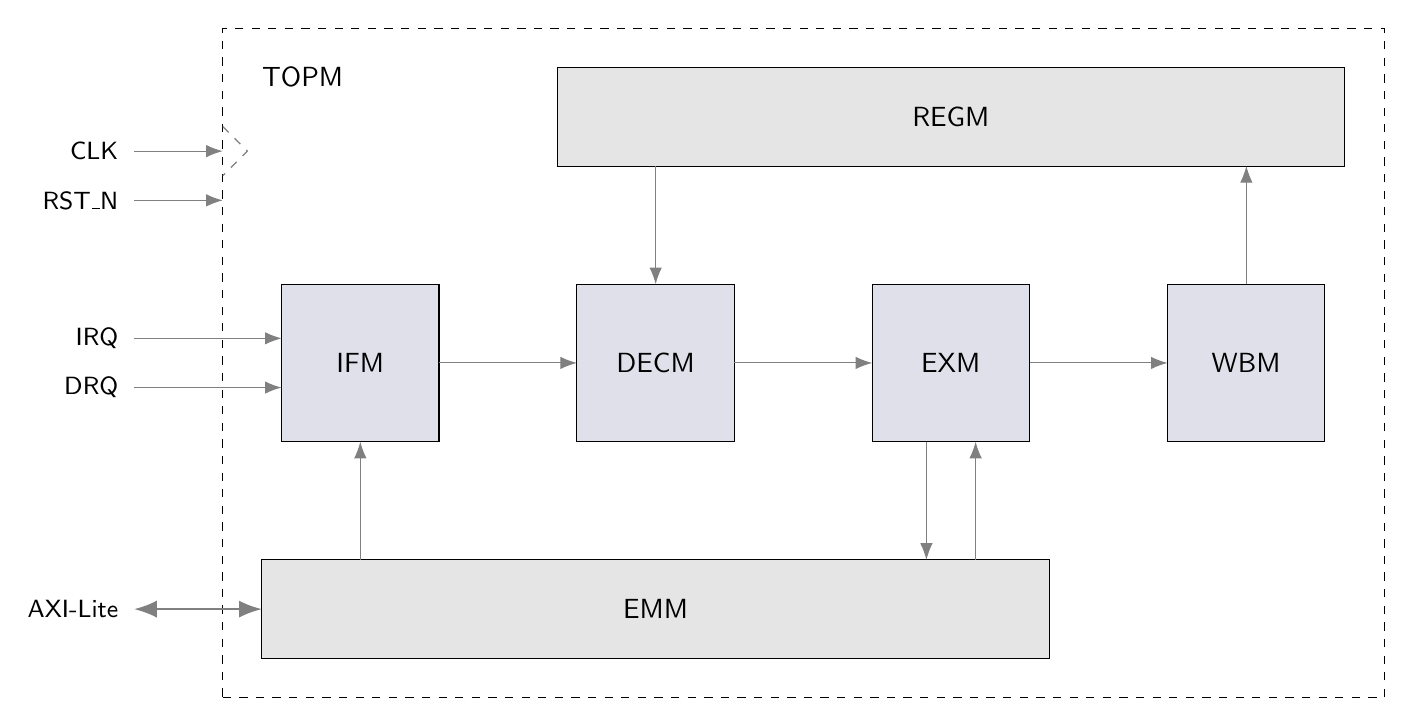
\begin{tikzpicture}[scale=1.25, draw=gray, inner sep=0, outer sep=0]
  \node[rectangle, draw=black,
    minimum height = 1.25cm,
    minimum width = 10cm,
    fill = gray!20] (EMM) at (6, -2.5) {EMM};
  \node[rectangle, draw=black,
    minimum height = 2cm,
    minimum width = 2cm,
    fill = blue!20!gray!20] (IFM) at (3, 0) {IFM};
  \node[rectangle, draw=black,
    minimum height = 2cm,
    minimum width = 2cm,
    fill = blue!20!gray!20] (DECM) at (6, 0) {DECM};
  \node[rectangle, draw=black,
    minimum height = 1.25cm,
    minimum width = 10cm,
    fill = gray!20] (REGM) at (9, 2.5) {REGM};
  \node[rectangle, draw=black,
    minimum height = 2cm,
    minimum width = 2cm,
    fill = blue!20!gray!20] (EXM) at (9, 0) {EXM};
  \node[rectangle, draw=black,
    minimum height = 2cm,
    minimum width = 2cm,
    fill = blue!20!gray!20] (WBM) at (12, 0) {WBM};

  \draw[->] (IFM.east) -- (DECM.west);
  \draw[->] (DECM.east) -- (EXM.west);
  \draw[->] (EXM.east) -- (WBM.west);

  \draw[<-] (IFM.south) -- (IFM.south|- EMM.north);

  \draw[->] ([xshift=-0.25cm]EXM.south) -- ([xshift=-0.25cm]EXM.south |- EMM.north);
  \draw[<-] ([xshift=0.25cm]EXM.south) -- ([xshift=0.25cm]EXM.south |- EMM.north);

  \draw[<-] (DECM.north) -- (DECM.north |- REGM.south);
  \draw[->] (WBM.north) -- (WBM.north |- REGM.south);

  % surrounding rectangle
  \node[dashed, draw=black, align=center, inner sep=0.5cm, fit=(EMM) (IFM) (DECM) (EXM) (WBM) (REGM)] (border) {};
  \node[anchor=north west, inner sep=0.5cm] (border-text) at (border.north west) {TOPM};

  % external interface
  \node (irq) at ([yshift=0.25cm]IFM.west) {};
  \node (drq) at ([yshift=-0.25cm]IFM.west) {};
  \node (axi) at (EMM.west) {};
  \node (clk) at ([yshift=-1.25cm]border.north west) {};
  \node (rst) at ([yshift=-1.75cm]border.north west) {};

  \node (extend) at ([xshift=-1.5cm]irq.center) {};

  \draw[->] (clk.center -| extend.center) node[left=0.2cm, anchor=east]{\small CLK} -- (clk.center);
  \draw[->] (rst.center -| extend.center) node[left=0.2cm, anchor=east]{\small RST\_N} -- (rst.center);
  \draw[->] (irq.center -| extend.center) node[left=0.2cm, anchor=east]{\small IRQ} -- (irq.center);
  \draw[->] (drq.center -| extend.center) node[left=0.2cm, anchor=east]{\small DRQ} -- (drq.center);
  \draw[<->, thick] (axi.center -| extend.center) node[left=0.2cm, anchor=east]{\small AXI-Lite} -- (axi.center);

  % clk triangle
  \draw[-, dashed] ([yshift=0.25cm]clk.center) -- ([xshift=0.25cm]clk.center) -- ([yshift=-0.25cm]clk.center);

\end{tikzpicture}
}

    \caption{Schematic view of the architecture of ECAP5-DPROC}
    \label{fig:architecture}
\end{figure}

  The design is split into the following functional modules :
  \begin{itemize}
    \vspace{-0.5em}
    \item The \textbf{Top Module} (TOPM) which integrates all other modules.
    \item The \textbf{External Memory Module} (EMM), in charge of accessing memory and peripherals.
    \vspace{-0.5em}
    \item The \textbf{Instruction Fetch Module} (IFM), in charge of implementing the instruction fetch stage.
    \vspace{-0.5em}
    \item The \textbf{Decode Module} (DECM), in charge of implementing the decode stage.
    \vspace{-0.5em}
    \item The \textbf{Register Module} (REGM), implementing the internal registers.
    \vspace{-0.5em}
    \item The \textbf{Execute Module} (EXM), in charge of implementing the execute stage.
    \item The \textbf{Write-Back Module} (WBM), in charge of implementing the write-back stage.
  \end{itemize}
\end{content}

\newpage

\section{Top Module}

\begin{content}
  Handshaking and bubbling
\end{content}

\newpage

\section{External Memory Module}
\newpage

\section{Instruction Fetch Module}
\newpage

\section{Decode Module}
\newpage

\section{Register Module}

\begin{figure}[h!]
    \centering
    \vspace{1em}
\scalebox{0.85}{
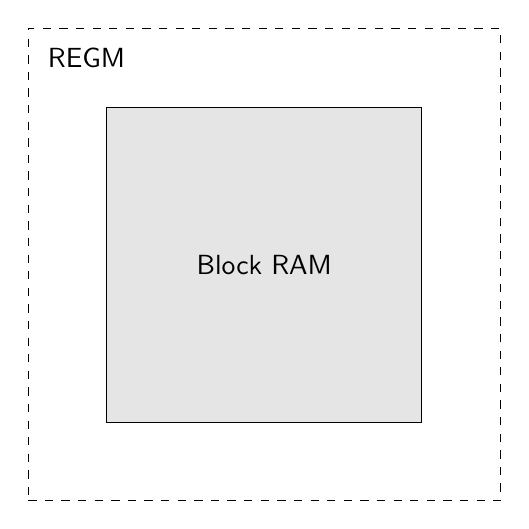
\begin{tikzpicture}[scale=1.25, draw=gray, inner sep=0, outer sep=0]
  \node[rectangle, draw=black,
    minimum height = 4cm,
    minimum width = 4cm,
    fill = gray!20] (BRAM) at (6, 2.5) {Block RAM};

  \node[dashed, draw=black, align=center, inner sep=1cm, fit=(BRAM)] (border) {};
  \node[anchor=north west, inner sep=0.25cm] (border-text) at (border.north west) {REGM};
\end{tikzpicture}
}

    \caption{Schematic view of the Register Module}
    \label{fig:regm}
\end{figure}

\newpage

\section{Execute Module}
\newpage

\section{Write-Back Module}
\newpage

\section{Debug}
\newpage


\end{document}
